\documentclass[11pt]{article}

% Page geometry and typography
\usepackage[margin=1in]{geometry}
\usepackage{microtype}
\usepackage{parskip}       % no paragraph indent, add vertical space
\usepackage{setspace}      % adjust spacing if needed

% Math and symbols
\usepackage{amsmath, amssymb, amsfonts}
\usepackage{siunitx}

% Figures and tables
\usepackage{graphicx}
\usepackage{subcaption}
\usepackage{booktabs}
\usepackage{caption}
\captionsetup{font=small, labelfont=bf}
\usepackage{float}         % for [H] placement

% Lists and compact spacing
\usepackage{enumitem}
\setlist{nosep}

% Links
\usepackage[hidelinks]{hyperref}

% References (optional: swap to biblatex if preferred)
\usepackage[numbers]{natbib}

\usepackage[table]{xcolor}
\definecolor{gain}{HTML}{D5F5D5}
\definecolor{loss}{HTML}{F8D2D2}
\definecolor{same}{HTML}{FFF4CC}

% Custom commands
\newcommand{\dataset}{GSN}
\newcommand{\loss}{\mathcal{L}}
\newcommand{\cls}{\text{NLL}}
\newcommand{\reg}{\text{SmoothL1}}

\title{Multitask Learning for Geometric Shape Classification and Counting}
\author{Grzegorz Krawczyk}
\date{\today}

\begin{document}
% \maketitle

\section{Dataset and EDA}
\textbf{Data:} 10k images (28$\times$28), 6 shape classes; exactly two non-zero counts per image; counts sum to 10.

\textbf{Split:} 9k train / 1k val.

\textbf{Sanity checks:} sum==10, exactly two non-zeros (no violations).

\textbf{Distributions:} class presence, count frequency, barplot of split into 135 classes (empty classes excluded).

\begin{figure}[H]
  \centering
  \begin{subfigure}{0.32\linewidth}
    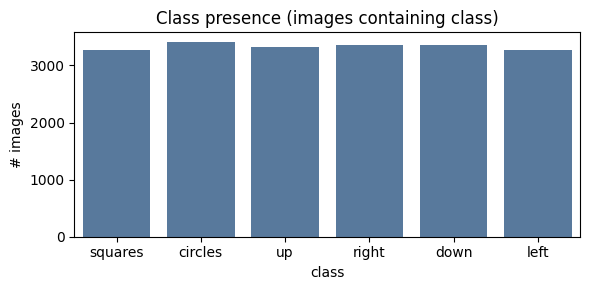
\includegraphics[width=\linewidth]{../plots/class-presence.png}
    \caption{Class presence}
  \end{subfigure}
  \begin{subfigure}{0.32\linewidth}
    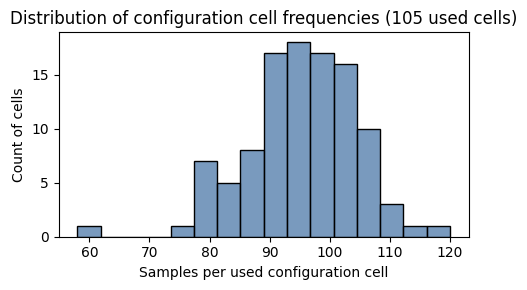
\includegraphics[width=\linewidth]{../plots/135-class-barplot.png}
    \caption{Pair frequency}
  \end{subfigure}
  \begin{subfigure}{0.32\linewidth}
    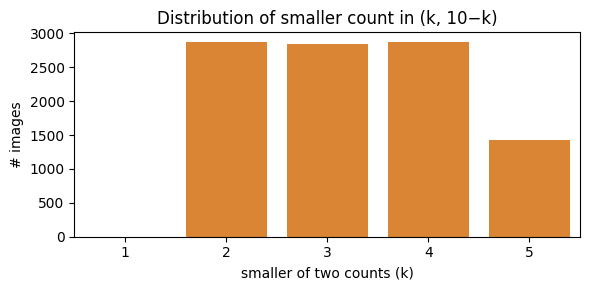
\includegraphics[width=\linewidth]{../plots/count-distribution.png}
    \caption{Count distribution}
  \end{subfigure}
  \caption{Dataset statistics.}
  \label{fig:dataset-stats}
\end{figure}

\subsection*{EDA \& Implications}
Shape presence is balanced across the six classes. Distribution of smaller count shows that occurances of counts 2-8 are also balanced. Counts 1 and 9 never appear, thus, only 105 of the 135 nominal configuration cells are populated. The per-configuration frequency barplot shows a dense central band (about 90--110 samples), a very short upper tail (few cells above 110), and a broader lower tail (many cells in 80--89). There is a pronounced gap separating the least-common outlier cell from the next least-common cell, indicating an isolated low-frequency outlier rather than a smoothly decaying tail. This represents moderate dispersion with one distinct low-frequency case.

\textbf{Implications:} no class or regression loss weighting; Macro-F1 reported to guard against configuration variance; watch out for elevated error in outlier configurations. Absence of $(1,9)$ splits may limit generalization to datasets containing such extremes.

\subsection*{Augmentations}

We use geometric augmentations that preserve label semantics on binary images: random horizontal flip, vertical flip, and 90° rotations, while adjusting the direction of the occuring triangle shapes appropriately. This increases effective sample diversity without increasing the dataset size on disk.

We omit photometric augmentations (brightness/contrast, Gaussian noise) because the dataset is synthetic and pixel values are binary; such changes introduce grayscale artifacts that do not reflect the data-generating process and can blur edges. We also omit random erasing, which often removes parts of small shapes and corrupts the count labels.

\section{Model}

The network consists of a fixed shared backbone and two task–specific heads.

\textbf{Backbone (shared feature extractor):} A stack of four 2D convolution layers (channel progression $1\!\rightarrow\!8\!\rightarrow\!16\!\rightarrow\!32\!\rightarrow\!64$) with $3\times3$ kernels, stride 1, padding 1 and ReLU activations, followed by flattening of the $64\times28\times28$ feature map and a fully connected layer to a 256‑dimensional latent representation (ReLU). This backbone is unchanged across experiments.

\textbf{Classification head:} A $256\!\rightarrow\!256$ fully connected layer with ReLU, dropout (probability $0.3$), then a $256\!\rightarrow\!135$ linear projection producing logits, converted to log‑probabilities by a LogSoftmax layer, yielding $\log p \in \mathbb{R}^{135}$.

\textbf{Regression head:} A $256\!\rightarrow\!256$ fully connected layer with ReLU, dropout (probability $0.3$), then a $256\!\rightarrow\!6$ linear layer producing raw continuous count estimates $\hat{\mathbf c}\in\mathbb{R}^6$.

\textbf{Outputs:} The forward pass returns $(\log p,\hat{\mathbf c})$ for each image.

\textbf{Joint loss:} Multitask training minimizes
\[
\mathcal{L} = \underbrace{\text{NLLLoss}(\log p, y_{135})}_{\mathcal{L}_{\text{cls}}}
+ \lambda_{\text{cnt}}\cdot\underbrace{\text{SmoothL1Loss}(\hat{\mathbf c}, \mathbf c)}_{\mathcal{L}_{\text{cnt}}}.
\]
Setting $\lambda_{\text{cnt}}=0$ yields classification‑only; omitting $\mathcal{L}_{\text{cls}}$ yields regression‑only. Dropout in each head regularizes the task‑specific layers without altering shared feature extraction.

\section{Results}
Training was performed with Adam (lr = $10^{-3}$), batch sizes $64$ (train) and $1\;000$ (validation), for up to $100$ epochs using early stopping on validation loss. The dataset split was fixed at $9\;000$ train / $1\;000$ validation samples. The global seed \texttt{torch.manual\_seed(1)} was set for reproducibility.

Training was performed separately for three settings of the model:
\begin{enumerate}[label=(\arabic*)]
  \item \textbf{Classification-only:} $\lambda_{\text{cnt}}=0$
  \item \textbf{Regression-only:} $\mathcal{L} = \mathcal{L}_{\text{cnt}}$ (classification loss ignored)
  \item \textbf{Multitask:} $\lambda_{\text{cnt}}=2$
\end{enumerate}

\begin{table}[H]
  \centering
  \small
  \begin{tabular}{lcccccccc}
    \toprule
    \textbf{Setting} & \textbf{Val Loss} & \textbf{Top-1} & \textbf{Macro-F1} & \textbf{RMSE} & \textbf{MAE} & \textbf{Best epoch} & \textbf{Epochs} & \textbf{Time} \\
    \midrule
    Cls-only  & 1.2859 & 45.4\% & 33.2\% & 3.2073 & 1.8862 & 34 & 45 & 122.71s \\
    Reg-only  & 0.1419 &  0.8\% &  0.1\% & 0.5831 & 0.3059 & 30 & 41 & 109.07s \\
    Multitask & 1.3835 & 52.5\% & 37.8\% & 0.5666 & 0.3089 & 30 & 41 & 111.68s \\
    \bottomrule
  \end{tabular}
  \caption{Training metrics across the three settings.}
\end{table}

\begin{table}[H]
  \centering
  \small
  \begin{tabular}{ccccccc}
    \toprule
    \textbf{Pair accuracy change} & $\square$ & $\bigcirc$ & $\bigtriangleup$ & $\rhd$ & $\bigtriangledown$ & $\lhd$ \\
    \midrule
    $\square$ & -- 
      & \cellcolor{gain} +6.35
      & \cellcolor{loss} -2.85
      & \cellcolor{gain} +11.11
      & \cellcolor{same}  0.00
      & \cellcolor{gain} +1.45 \\
    $\bigcirc$ 
      & \cellcolor{gain} +6.35 & -- 
      & \cellcolor{gain} +4.00
      & \cellcolor{loss} -4.22
      & \cellcolor{gain} +4.92
      & \cellcolor{same}  0.00 \\
    $\bigtriangleup$
      & \cellcolor{loss} -2.85
      & \cellcolor{gain} +4.00 & -- 
      & \cellcolor{same}  0.00
      & \cellcolor{gain} +13.43
      & \cellcolor{loss} -3.08 \\
    $\rhd$
      & \cellcolor{gain} +11.11
      & \cellcolor{loss} -4.22
      & \cellcolor{same}  0.00 & -- 
      & \cellcolor{same}  0.00
      & \cellcolor{same}  0.00 \\
    $\bigtriangledown$
      & \cellcolor{same}  0.00
      & \cellcolor{gain} +4.92
      & \cellcolor{gain} +13.43
      & \cellcolor{same}  0.00 & -- 
      & \cellcolor{same}  0.00 \\
    $\lhd$
      & \cellcolor{gain} +1.45
      & \cellcolor{same}  0.00
      & \cellcolor{loss} -3.08
      & \cellcolor{same}  0.00
      & \cellcolor{same}  0.00 & -- \\
    \bottomrule
  \end{tabular}
  \caption{Pairwise validation accuracies delta from classification-only to multitask setting.}
\end{table}

\begin{table}[H]
  \centering
  \small
  \begin{tabular}{ccccccc}
    \toprule
    \textbf{Classification-only} & $\square$ & $\bigcirc$ & $\bigtriangleup$ & $\rhd$ & $\bigtriangledown$ & $\lhd$ \\
    \midrule
    $\square$          & --      & 90.48\% & 95.71\% & 82.54\% & 93.75\% & 92.75\% \\
    $\bigcirc$         & 90.48\% & --      & 96.00\% & 98.59\% & 95.08\% & 95.31\% \\
    $\bigtriangleup$   & 95.71\% & 96.00\% & --      & 96.92\% & 86.57\% & 93.85\% \\
    $\rhd$             & 82.54\% & 98.59\% & 96.92\% & --      & 91.94\% & 96.97\% \\
    $\bigtriangledown$ & 93.75\% & 95.08\% & 86.57\% & 91.94\% & --      & 92.00\% \\
    $\lhd$             & 92.75\% & 95.31\% & 93.85\% & 96.97\% & 92.00\% & --      \\
    \bottomrule
  \end{tabular}
  \caption{Validation accuracies for shape pairs, classification-only setting.}
\end{table}

\begin{table}[H]
  \centering
  \small
  \begin{tabular}{ccccccc}
    \toprule
    \textbf{Multitask} & $\square$ & $\bigcirc$ & $\bigtriangleup$ & $\rhd$ & $\bigtriangledown$ & $\lhd$ \\
    \midrule
    $\square$          & --      &  96.83\% &  92.86\% & 93.65\% &  93.75\% & 94.20\% \\
    $\bigcirc$         & 96.83\% & --       & 100.00\% & 94.37\% & 100.00\% & 95.31\% \\
    $\bigtriangleup$   & 92.86\% & 100.00\% & --       & 96.92\% & 100.00\% & 90.77\% \\
    $\rhd$             & 93.65\% &  94.37\% &  96.92\% & --      &  91.94\% & 96.97\% \\
    $\bigtriangledown$ & 93.75\% & 100.00\% & 100.00\% & 91.94\% & --       & 92.00\% \\
    $\lhd$             & 94.20\% &  95.31\% &  90.77\% & 96.97\% &  92.00\% & --      \\
    \bottomrule
  \end{tabular}
  \caption{Validation accuracies for shape pairs, multitask setting.}
\end{table}

\begin{figure}[H]
  \centering
  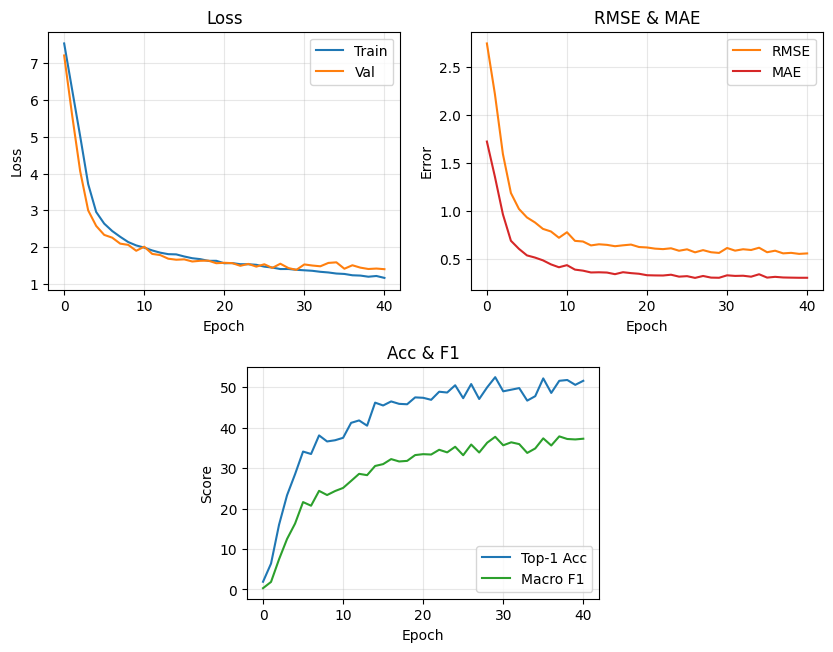
\includegraphics[width=0.75\linewidth]{../plots/multitask-training.png}
  \caption{Training plots for multitask setting.}
  \label{fig:cls-training}
\end{figure}

\begin{figure}[H]
  \centering
  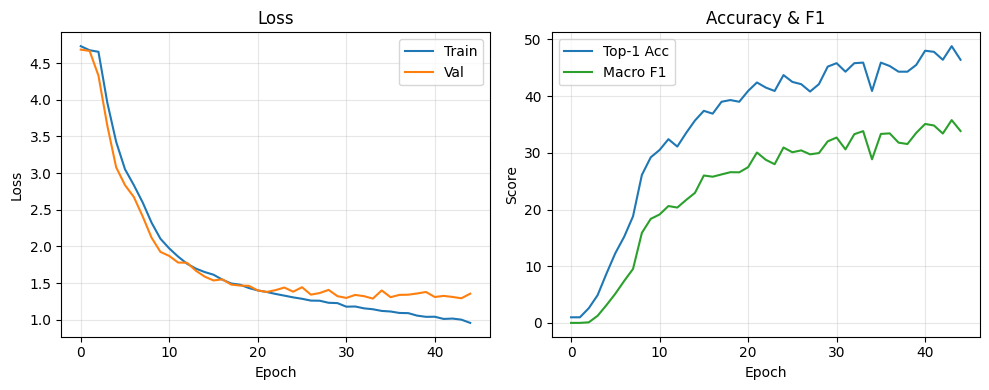
\includegraphics[width=0.75\linewidth]{../plots/classification-training.png}
  \caption{Training plots for classification-only setting}
  \label{fig:cls-training}
\end{figure}


\begin{figure}[H]
  \centering
  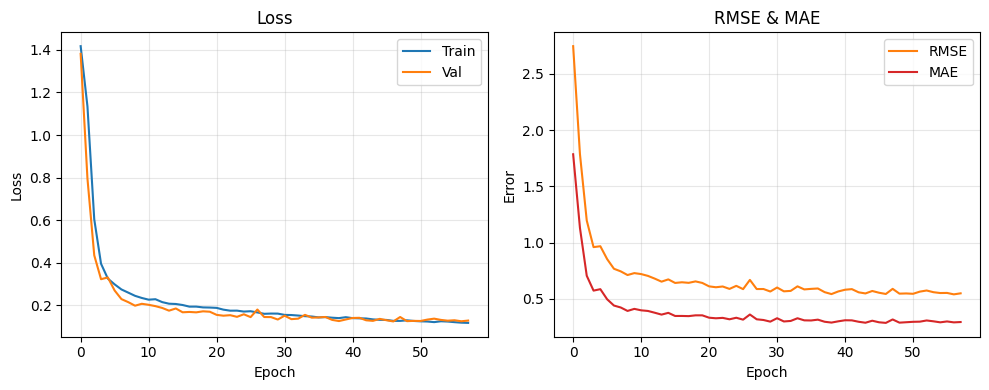
\includegraphics[width=0.75\linewidth]{../plots/regression-training.png}
  \caption{Training plots for regression-only setting.}
  \label{fig:cls-training}
\end{figure}

\section{Discussion}
Multitask learning produced clear net positive transfer. Joint training increased validation Top-1 accuracy by $7.1$ percentage points and Macro-F1 by $4.6$ points over the classification-only baseline. Remarkably, the multitask model also improved RMSE relative to the regression-only configuration ($0.5831 \rightarrow 0.5666$), indicating that classification supervision helped suppress larger counting errors.

Pairwise shape analysis shows concentrated gains in challenging orientation or mixed-shape combinations (e.g. up–down $+13.43$ pp, square-right $+11.11$ pp). These improvements suggest the count head encourages the backbone to encode finer spatial/orientation cues that also benefit discrimination. A small number of pairs (square-up, circle-right, up-left) declined modestly ($-3$ to $-4$ pp), consistent with mild gradient interference across tasks. Some pairs remained unchanged (already near high performance), supporting that auxiliary regression acts primarily as a regularizer where headroom existed.

Training dynamics reinforce this interpretation: the multitask model reached its best epoch earlier and exhibited slower overfitting than classification-only, reflecting stabilizing shared supervision. The chosen $\lambda_\text{cnt} = 2$ balanced initial loss scales (classification $\approx 3.4 \times$ regression), elevating regression’s influence enough to yield transfer without sacrificing primary classification accuracy.

Overall, gains in difficult orientation pairs and improved RMSE outweigh localized drops, making multitask learning well-suited for this dataset.

\bibliographystyle{unsrt}
% \bibliography{refs} % optional
\end{document}
